\section{Weight Diagnostics}
\label{ssec:balancetables}

Table~\ref{tab:baltab1} displays the differences between the weighted mean covariate values of the expansion region and the mean of the non-expansion region for our primary dataset and with the early expansion states excluded (calculated using our covariate adjustments). The weights presented here are from the H-SBW estimator. The values under each column of ``Primary'' and ``Early Excluded'' are in the following format: (unweighted difference, weighted difference). Additional results are available on request.

\begin{table}[ht]
\centering
    \caption{Balance Table}
    \label{tab:baltab1}
\begin{tabular}{lll}
  \hline
Variables & Preferred & Early Excluded \\ 
  \hline
Age: 19-29 Pct & (-0.34, -0.34) & (-0.64, -0.22) \\ 
  Age: 30-39 Pct & (0.36, 0.17) & (-0.08, 0.27) \\ 
  Age: 40-49 Pct & (0.19, -0.3) & (0.07, -0.36) \\ 
  Avg Adult to Household Ratio & (11.29, -0.04) & (3.33, 0.04) \\ 
  Citizenship Pct & (-3.61, -1.59) & (-0.24, -1.44) \\ 
  Disability Pct & (-1.45, 0.52) & (-0.18, 0.62) \\ 
  Educ: HS Degree Pct & (-3.37, 0.54) & (-1.03, 0.60) \\ 
  Educ: Less than HS Pct & (-0.37, 0.83) & (-1.24, 0.73) \\ 
  Educ: Some College Pct & (-0.35, 0.40) & (0.44, 0.70) \\ 
  Female Pct & (-0.34, -0.64) & (-0.25, -1.00) \\ 
  Foreign Born Pct & (7.6, 2.00) & (1, 1.98) \\ 
  Uninsured Pct 2011 & (-3.08, 0.05) & (-2.53, 0.96) \\ 
  Uninsured Pct 2012 & (-3, -0.05) & (-4.28, -0.88) \\ 
  Uninsured Pct 2013 & (-2.99, -0.05) & (-3.92, -0.52) \\ 
  Hispanic Pct & (4.46, 1) & (-1.35, 1) \\ 
  Inc Pov: $<$ 138 Pct & (-2.05, 0.63) & (-1.38, 0.09) \\ 
  Inc Pov: 139-299 Pct & (-2.45, 0.65) & (-1.16, 0.83) \\ 
  Inc Pov: 300-499 Pct & (-0.59, -0.18) & (-0.22, -0.69) \\ 
  Inc Pov: 500 + Pct & (5.58, -1.3) & (3.07, -1.01) \\ 
  Married Pct & (-0.76, -0.43) & (-0.34, -0.67) \\ 
  Children: Missing Pct & (-3.25, -1.00) & (-2.01, -0.11) \\ 
  Children: One Pct & (0.70, -0.14) & (0.35, -0.07) \\ 
  Avg Pop Growth & (-0.09, -0.21) & (0.25, 0.39) \\ 
  Race: White Pct & (-4.02, 1) & (0.09, 1.01) \\ 
  Republican Governor 2013 & (-64.78, -25) & (-54.46, -24.87) \\ 
  Republican Lower Leg Control 2013 & (-74.72, -25) & (-56.67, -23.6) \\ 
  Republican Total Control 2013 & (-71.3, -25) & (-56.47, -25) \\ 
  Student Pct & (0.25, -0.5) & (0.18, -0.18) \\ 
  Children: Three or More Pct & (0.00, -0.21) & (-0.11, -0.20) \\ 
  Children: Two Pct & (0.76, -0.31) & (-0.03, -0.58) \\ 
  Unemployed Pct 2011 & (0.82, 0.15) & (0.62, 0.11) \\ 
  Unemployed Pct 2012 & (0.63, -0.03) & (0.54, 0.02) \\ 
  Unemployed Pct 2013 & (0.42, -0.15) & (0.25, -0.16) \\ 
  Urban Pct & (8.28, -2.00) & (2.79, -2.00) \\ 
   \hline
\end{tabular}
\end{table}

Figure~\ref{fig:weightsbystatec2} display the weights summed by states when excluding the early expansion states for the H-SBW and BC-HSBW estimators.

\begin{figure}[H]
\begin{center}
    \caption{Total weights summed by state, early expansion removed}
    \label{fig:weightsbystatec2}
    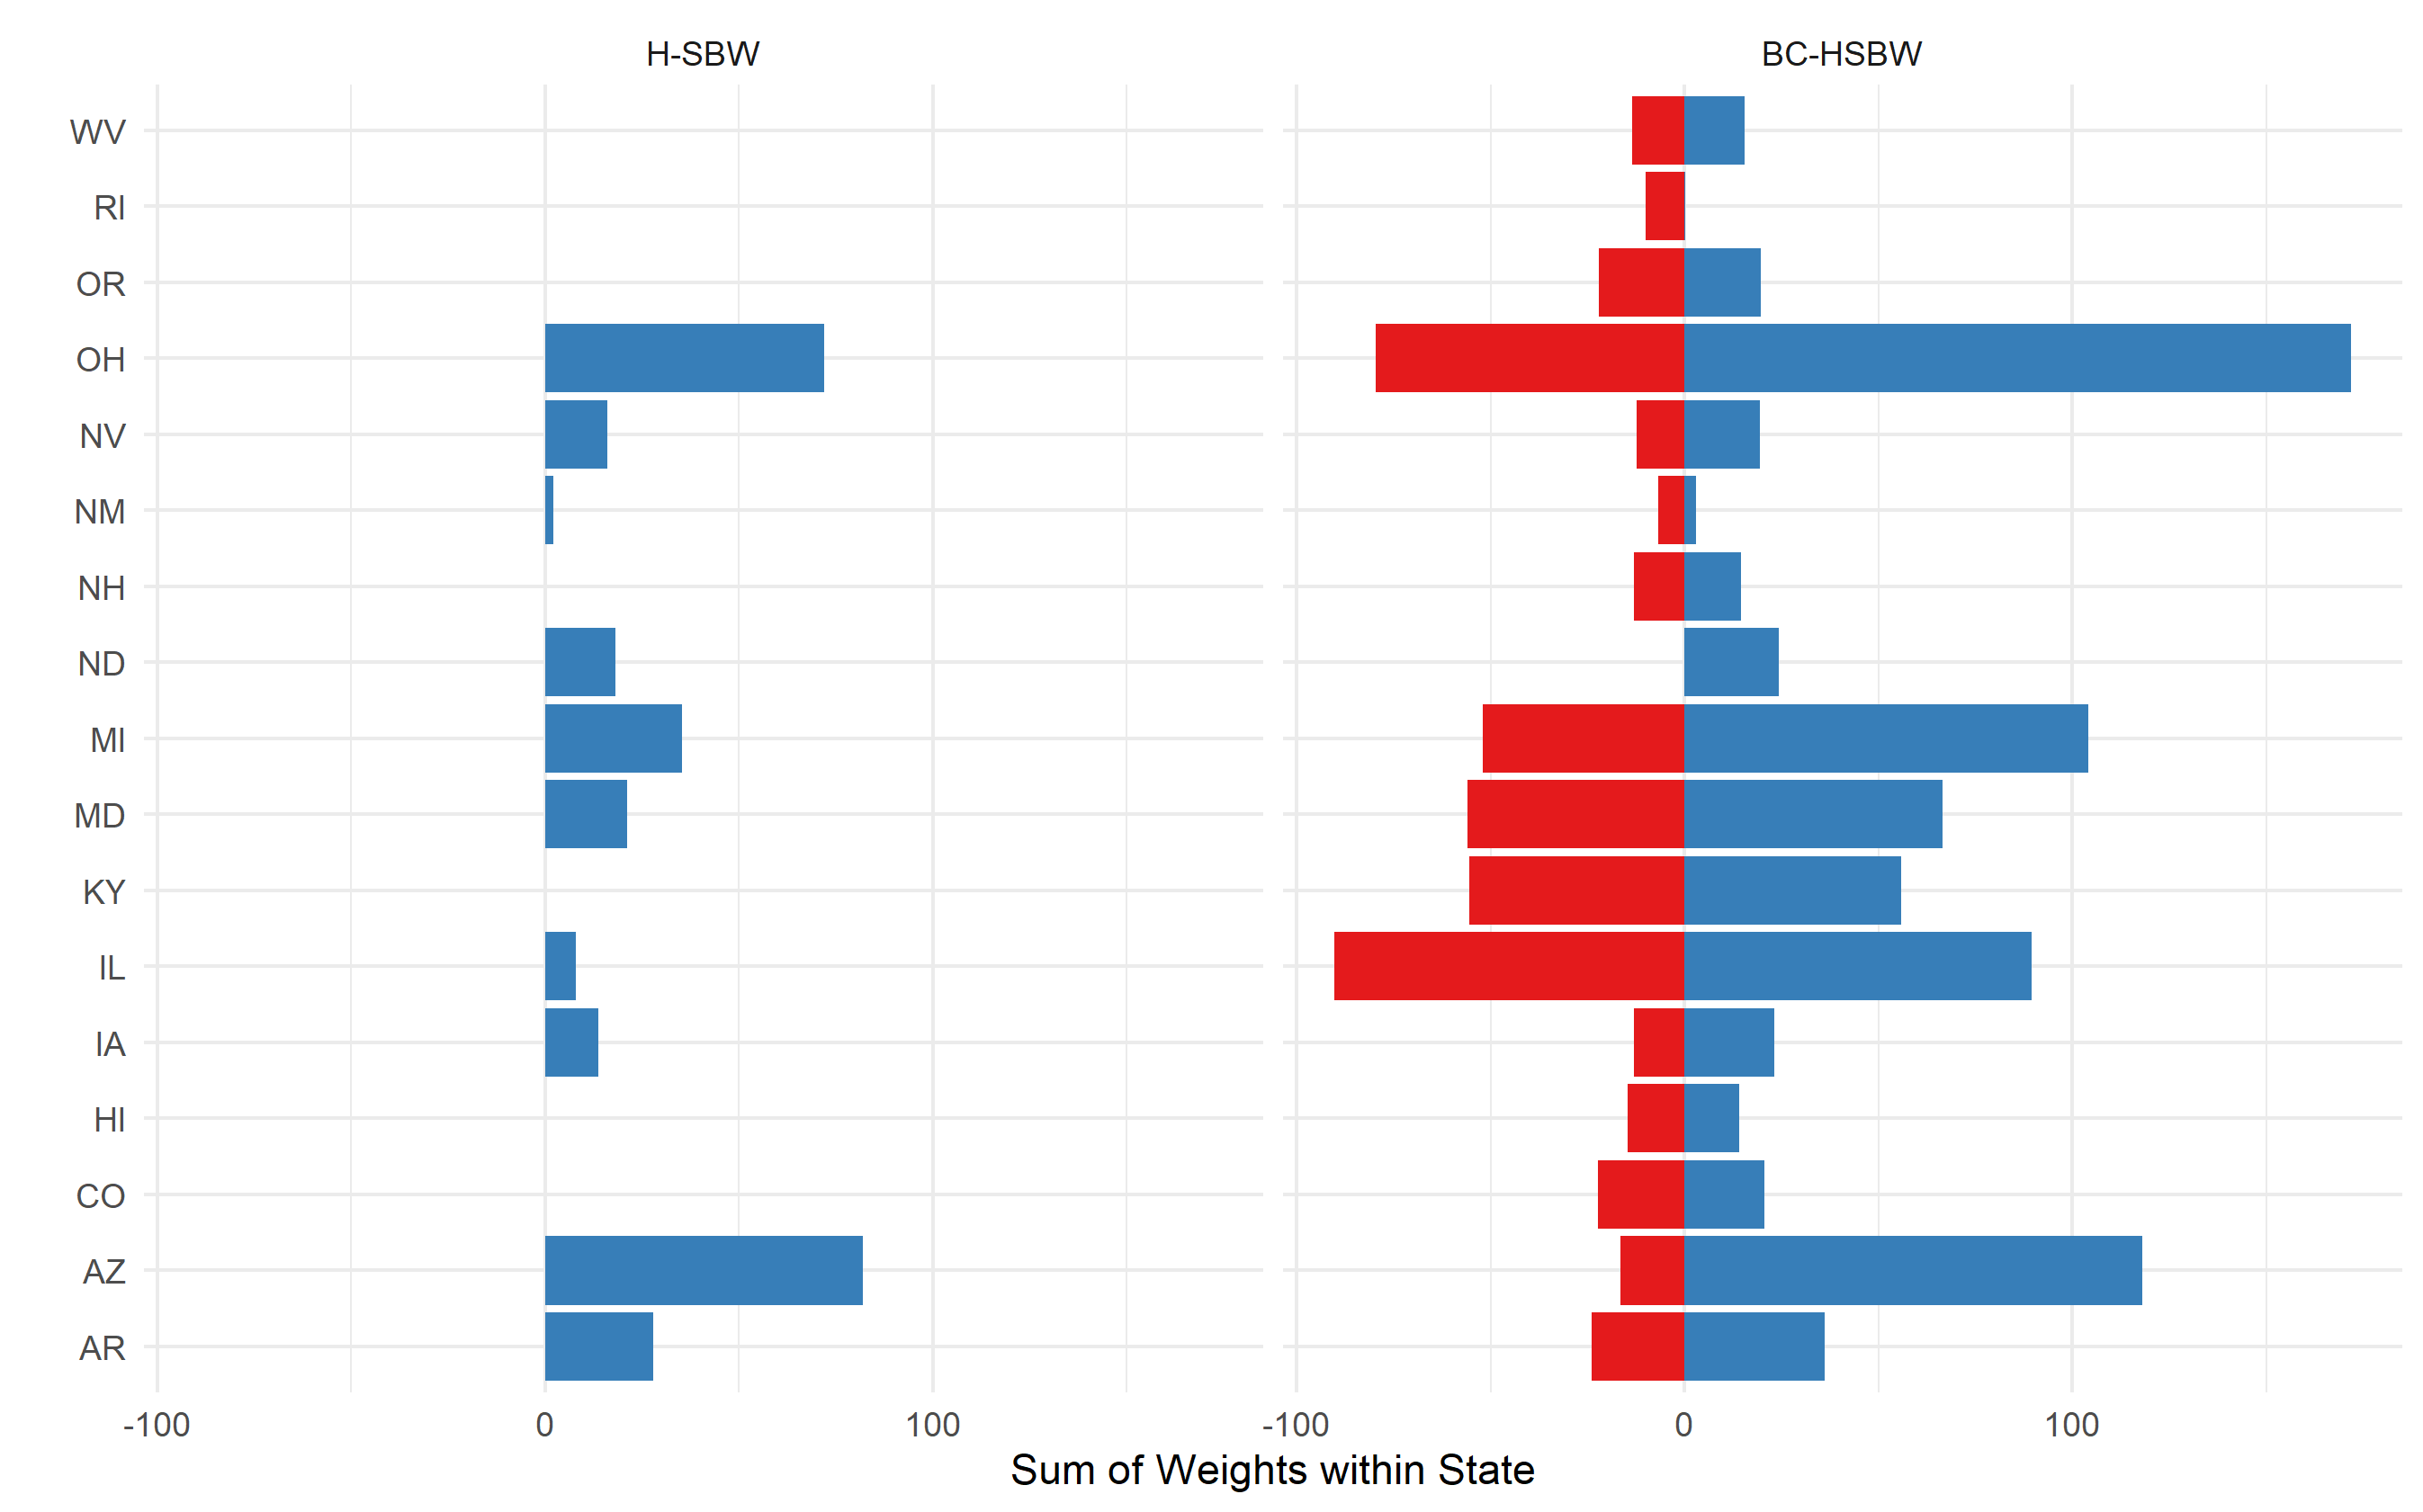
\includegraphics[scale=0.6]{01_Plots/weights-by-state-hsbw-c2.png}
\end{center}
\end{figure}
